\documentclass[12pt]{report}
\usepackage[utf8]{inputenc}
\setcounter{tocdepth}{3}
\setcounter{secnumdepth}{3}
\usepackage{tgbonum}
\usepackage[english]{babel}
\usepackage{graphicx}
\usepackage{amsmath}
\usepackage{amssymb}
\usepackage[hidelinks]{hyperref}
\usepackage{epsf}
\usepackage{float}
\usepackage{mathpazo}
\usepackage{pifont}
\usepackage{color}
\definecolor{mygreen}{RGB}{70, 180, 90}
\definecolor{mylilas}{RGB}{255, 117, 45}
\definecolor{cadr}{rgb}{0.89, 0.0, 0.13}
\definecolor{myblue}{RGB}{0, 102, 204}
\usepackage{caption}
\usepackage{subcaption}
\usepackage{subfloat}
\usepackage{tocloft}
\setlength{\cftbeforesecskip}{5pt}
\usepackage
[
a4paper,% other options: a3paper, a5paper, etc
left=3cm,
right=3cm,
top=3cm,
bottom=3cm,
]{geometry}
%\geometry{hmargin=3.5cm, vmargin=2.5cm}
\usepackage{fancyhdr}
\pagestyle{fancy}
\fancyhf{}
\rfoot{\thepage}
\renewcommand{\headrulewidth}{0pt}
\usepackage{color}
\graphicspath{{figures/}}
\usepackage{graphicx}
\usepackage{wrapfig}
\usepackage{graphicx}
\usepackage{multicol}
\usepackage{enumitem}
\usepackage{xcolor}
\usepackage{framed}
\usepackage{bm}
\definecolor{shadecolor}{RGB}{139, 231, 3}
\usepackage{epigraph}

\usepackage{mathpazo}
\usepackage[framemethod=TikZ]{mdframed}
\usepackage{lipsum}

\usepackage{color}
\definecolor{color-box-border-equation}{RGB}{200,200,200}
\definecolor{color-box-background-equation}{RGB}{250,250,250}

\definecolor{color-box-border-code}{RGB}{54,119,168}
\definecolor{color-box-background-code}{RGB}{236,245,255}

\mdfdefinestyle{equation-frame}{%
    linecolor=color-box-border-equation,
    outerlinewidth=1pt,
    roundcorner=10pt,
    innertopmargin=\baselineskip,
    innerbottommargin=\baselineskip,
    innerrightmargin=20pt,
    innerleftmargin=20pt,
    backgroundcolor=color-box-background-equation}
    
\mdfdefinestyle{exercise-frame}{%
    linecolor=color-box-border-code,
    outerlinewidth=1pt,
    roundcorner=10pt,
    innertopmargin=\baselineskip,
    innerbottommargin=\baselineskip,
    innerrightmargin=20pt,
    innerleftmargin=20pt,
    backgroundcolor=color-box-background-code}

\usepackage{pifont}

\usepackage{tcolorbox}
\definecolor{mycolor}{rgb}{0.122, 0.435, 0.698}

\newtcbox{\mb}{nobeforeafter,colframe=mycolor,colback=mycolor!10!white,boxrule=0.5pt,arc=4pt,
  boxsep=0pt,left=6pt,right=6pt,top=3pt,bottom=3pt,tcbox raise base}

\usepackage{eso-pic}
\newcommand\BackgroundPic{%
\put(-50,-0){%
\parbox[b][\paperheight]{\paperwidth}{%
\vfill
\centering
\includegraphics[height=\paperheight,%
keepaspectratio]{figures/cover.png}%
\vfill
}}}

%\usepackage{emerald}
\usepackage[T1]{fontenc}

\usepackage{anyfontsize}
\usepackage{t1enc}
\newcommand{\heart}{\ensuremath\varheartsuit}
\usepackage{tikz}
\usetikzlibrary{positioning}

% CHAPTER STYLE =================================================

\makeatletter
\def\thickhrulefill{\leavevmode \leaders \hrule height 1ex \hfill \kern \z@}
\def\@makechapterhead#1{%
  \vspace*{10\p@}%
  {\parindent \z@ \raggedleft \reset@font
            \scshape \@chapapp{} \thechapter
        \par\nobreak
        \interlinepenalty\@M
    \Huge \bfseries #1\par\nobreak
    %\vspace*{1\p@}%
    %\hrulefill
    \par\nobreak
    \vskip 50\p@
  }}
\def\@makeschapterhead#1{%
  \vspace*{10\p@}%
  {\parindent \z@ \raggedleft \reset@font
            \scshape \vphantom{\@chapapp{} \thechapter}
        \par\nobreak
        \interlinepenalty\@M
    \Huge \bfseries #1\par\nobreak
    %\vspace*{1\p@}%
    %\hrulefill
    \par\nobreak
    \vskip 50\p@
  }}

\begin{document}

% TITLE PAGE ====================================================

\begin{titlepage}
\AddToShipoutPicture*{\BackgroundPic}
\ \\[4cm]
{\sffamily \color{white}
\begin{center}
\fontsize{76}{10}\selectfont \fontfamily{qcr}\selectfont Fluid

\vskip 5\p@

\fontsize{55}{10}\selectfont \fontfamily{qcr}\selectfont Toolbox

\vskip 10\p@

%\fontsize{25}{10} \selectfont \fontfamily{augie}\selectfont with Python

\end{center}
}
\vfill
{\fontsize{20}{20}\color{white}\sffamily Kamila Zdybał \hfill\color{white} Zürich, 2025}

{\fontsize{10}{10}\color{white}\sffamily \href{https://kamilazdybal.github.io/}{\texttt{kamilazdybal.github.io}}}
\end{titlepage}


% EX LIBRIS PAGE ================================================

\thispagestyle{empty}
\begin{center}
\vspace*{1cm}
\includegraphics[width = 80mm]{ex_libris_arduino.jpg}

\vspace*{1cm}

{\fontsize{18}{10}\selectfont \fontfamily{pbk}\selectfont E X \,\, L I B R I S $\cdotp$ K A M I L A}

\vspace*{2cm}

Copyright \textcopyright \, K. Zdybał, 2025

For more projects similar to this one

visit my personal website: \verb|kamilazdybal.github.io|

or visit me on GitHub: \verb|@kamilazdybal|

You can contact me with any thoughts, suggestions, or corrections:

\verb|kamilazdybal at gmail dot com|

\vspace*{0.6cm}

This document will be alive for quite some time. 

I will be coming back to it to add or improve things. 

You can always access the newest version through my website.

\vspace*{1.8cm}

\verb|Fluid Toolbox|

\verb|version 1.1|

Typeset with \ding{170} for \LaTeX

\vspace*{1.8cm}

\noindent This work is licensed under the Creative Commons

Attribution-NonCommercial-ShareAlike 4.0 International 

(CC BY-NC-SA
4.0) license.
\end{center}

\setlength{\parskip}{0.6em}
\setlength{\parindent}{0cm}

\chapter*{Preface}
\thispagestyle{empty}
\chaptermark{Preface}

\rightline{{\rm \textit{``Use it well.''}}}

\rightline{{\rm --- Prof. Albus Dumbledore}}

\texttt{\textbf{Fluid Toolbox}} is a collection of human-readable, pseudo-random study notes that inspire you to think deeper about various fluid dynamics concepts. It is meant to be used complementary to the regular textbook since it may provide additional insights, but it will not substitute the thoroughness of a standard course in the subject. I believe that working side-by-side with a course it can become a useful toolbox of concepts that are ready-to-understand and ready-to-use.

\textbf{Why is this text created?}

I had a goal of collecting in one place the most important fluid dynamics concepts, as well as some prerequisites to studying fluid dynamics. Much of the knowledge presented here comes from my search for understanding that I was often missing when reading textbooks, and which was difficult to find in a way that would be engaging, illustrative, and would make intuitive sense to me. Some of the understanding presented here comes from my personal explorations and thinking on the subject, some of it comes from sources that I found very helpful -- I will make references to those as we go. I have hopes that this document will become a helpful resource that you have been looking for. Above all, I will know that it was worth writing it if you enjoy the journey of reading and learning from it!

\textbf{Some of my thoughts on learning}

I believe in the quote by Richard Feynman: \textit{Study hard what interests you the most in the most undisciplined, irreverent, and original manner possible.} I will sometimes ask a brain-teasing question or challenge you to \textit{pause and ponder}. In your own learning, do challenge yourself, and don't let your imagination be limited by simply following pages of any textbook! When learning a new subject, it's simply not enough to read a textbook or watch a lecture; those are both easy tasks to do. When you become a spectator in the studying process, it's easy to fool yourself that you understood something. The real learning and understanding comes when it's only you, your head, and a blank piece of paper. It is only when you have a chance to take action in your recall of information that you can really use your knowledge and test your deep understanding. Oh, and by the way... Programming is a great way to roll your sleeves and put things into action. So is teaching others!\footnote{And so my sneaky goal is to learn some fluid dynamics writing this document!}

\newpage
\thispagestyle{empty}
\tableofcontents

\newpage
\chapter*{Acknowledgements}
\thispagestyle{empty}
\chaptermark{Ack}

{\fontsize{12}{12}\rightline{\textit{I am grateful to all people I encountered in my life}}}

\vspace*{0.5cm}

{\fontsize{12}{12}\rightline{\textit{who supported my passion for studying fluid motion.}}}

\vspace*{0.5cm}

{\fontsize{12}{12}\rightline{\textit{Among the first ones were Y. Çengel and J. Cimbala}}}

\vspace*{0.5cm}

{\fontsize{12}{12}\rightline{\textit{in their inspiring fluid mechanics textbook.}}}

\vspace*{2cm}
\rightline{{\rm \textit{Zürich, Switzerland, 2025}}}


\newpage

% - - - - - - - - - - - - - - - - - - - - - - - - - - - - - - - - - - - - - - - - - - - - - - - - 
\chapter{Changes} \label{chap:changes}

\rightline{{\rm \textit{Ch-ch-ch-ch-changes}}}
\rightline{{\rm \textit{Turn and face the strange}}}
\rightline{{\rm \textit{Ch-ch-changes}}}
\rightline{{\rm \textit{There's gonna have to be a different man}}}

\rightline{{\rm --- David Bowie}}

In studying fluid motion, we are inherently interested in \textbf{change} in various quantities associated with the fluid. For example, simply because of fluid moving around, its local density or its local temperature might change. With that perspective, the main goal of the science of fluid dynamics is to describe and then calculate that change. Much of the time, we would like to know how flow affects various fluid properties such as its density, pressure, temperature, or even things like mixture composition in multicomponent fluids.
In this Chapter, I discuss the most fundamental building block for talking about change -- \textbf{a derivative}. I hope to show you just how expressive derivatives are in terms of the various types of processes that they can describe!

\section{Derivatives model change}

\textbf{Change} is mathematically modeled by \textbf{derivatives}. A derivative explains how much one variable, say $\varphi$, changes when we change some other variable, say $\psi$, and we express this in mathematical terms as
\begin{equation*}\label{eq:change-d}
\frac{d \varphi}{d \psi} \, ,
\end{equation*}
where the letter $d$ stands for \textit{the change of...} and is later followed by the variable that we are speaking of. So really the above ratio means that there is \textit{this much} change in variable $\varphi$ per \textit{this much} change in variable $\psi$. You can also think of this ratio as \textit{this much} change in variable $\varphi$ per \textit{unit} change in variable $\psi$.

In fluid dynamics, you will find that we are most interested in two types of change: \textit{change in time} and \textit{change in space}. Since we live in a 3D space, with Cartesian coordinates $x$, $y$, and $z$, with a time arrow ($t$), it is justifiable why these two have the biggest popularity, right? Therefore, you will most often encounter $dt$, or $dx$, $dy$, and $dz$, in the denominator of various forms of derivatives.

Let's take pressure, $p$, as an example. When we write
\begin{equation*}\label{eq:change-p}
\frac{d p}{d t} \, ,
\end{equation*}
you can read this as: there is this much change in $p$ per this much change in $t$. Here, we have implicitly assumed that $p = p(t)$, that is, that pressure is only a function of time (and not space).
Similarly, you may encounter expressions like
\begin{equation*}\label{eq:change-p}
\frac{d p}{d x} \,  , \,\, \frac{d p}{d y} \, , \,\, \text{and} \,\, \frac{d p}{d z} \, ,
\end{equation*}
which you can read as: change in $p$ per change in $x$, or $y$, or $z$. 
Here, the assumption was that $p = p(x)$, or $p = p(y)$, or $p = p(z)$, respectively.

The above are what we call \textit{ordinary derivatives}. They assume that the variable can change with respect to only one independent variable. But this does not always need to be the case. 

There is also another mathematical expression for a derivative and it is
\begin{equation*}\label{eq:change-partial}
\frac{\partial \varphi}{\partial \psi} \, .
\end{equation*}
The operator $\partial$ (called ''partial`` or ''del``) also stands for \textit{the change of...} but it also gives you a hint that the variable $\varphi$ can change with the change of variables other than $\psi$. Perhaps it can also change with some $\zeta$ and $\chi$, even though in this particular ratio from above we are only interested in the change with respect to $\psi$.

These are called \textit{partial derivatives}. If a variable is a function of more than one independent variable, say $p = p(x,t)$, we are no longer allowed to use ordinary derivatives to be mathematically precise\footnote{Although we all allow ourselves to be mathematically sloppy sometimes! And that's alright, as long as we remember how to be precise if needed.}. Therefore, if $p = p(x,t)$, and we want to express the change of $p$ with respect to time, we have to write
\begin{equation*}\label{eq:change-partial}
\frac{\partial p}{\partial t}
\end{equation*}
and we can no longer write
\begin{equation*}\label{eq:change-partial}
\frac{d p}{d t} \, .
\end{equation*}


There are what we call \textit{higher-order derivatives}, which can look like this:
\begin{equation*}\label{eq:change-partial-2nd}
\frac{\partial^2 \varphi}{\partial \psi^2} \, .
\end{equation*}
What is their meaning? Well, we can also re-write the above as
\begin{equation*}\label{eq:change-partial}
\frac{\partial}{\partial \psi} \frac{\partial \varphi}{\partial \psi} \, ,
\end{equation*}
and this way it's easier to see that this must have the interpretation of measuring how much the very change in $\varphi$ is changing! In other words, we are describing how the quantity 
\begin{equation*}\label{eq:second-derivative}
\frac{\partial \varphi}{\partial \psi}
\end{equation*}
changes with the change to $\psi$. 

\section{Mixing derivatives signals various transport processes} \label{sec:changes:mixing-derivatives}

The really exciting part begins when we equate derivatives with respect to one quantity to derivatives with respect to other quantity. For instance, we can write that
\begin{equation}\label{eq:dt-propto-dx}
\frac{\partial p}{\partial t} \propto \frac{\partial p}{\partial x}
\end{equation}
for a particular point in space and time, and where the pressure, $p = p(x, t)$.

At first glance, it seems rather bizarre to say that a variable's change in time is proportional to its change in space. In the end, I can imagine a function that varies in space and varies in time, but those variations are completely independent of each other. So what does creating a link between space and time mean...? Let's think about this a little more!

First, we have to come to an agreement where exactly are we measuring $\partial p / \partial t$. With the continuum assumption of fluid dynamics, this is always some point in space, say $Q$. Now that we have selected $Q$, let's look at its local neighborhood to determine how does $p$ vary spatially there. This is what the term $\partial p / \partial x$ describes: How much change in $p$ is there along the spatial $x$-direction? But just the sheer existence of that change does not yet mean that our point $Q$ is going to experience any of it as time goes by! That change simply \textit{is}. If we now wanted it to affect our point $Q$, we need to somehow transport that change over to the location $Q$. And fluid's velocity is a great conveyor of that change! In this case, we have just one spatial dimension, therefore the fluid velocity vector $\vec{\bm{V}} = \langle u \rangle$. If we assume that the velocity component in the $x$-direction, $u$, is the constant of proportionality in Eq.~(\ref{eq:dt-propto-dx}), then we have just described an advection of $p$, which in its full form reads
\begin{equation}\label{eq:advection-of-p}
\frac{\partial p}{\partial t} = - u \frac{\partial p}{\partial x} \, .
\end{equation}
Equating the term $- u \partial p / \partial x$ to the temporal derivative, $\partial p / \partial t$, tells us how much of the spatial change in $p$ is being ``slided over'' to the fixed point in space, $Q$. And the strength of that ``sliding over'' is measured by the velocity component, $u$.

Turns out, the link between time and space, embedded in Eq.~(\ref{eq:advection-of-p}), is necessary when we assume fluid's \textit{movement}. 
As we have seen, a moving fluid can alter a point in time by bringing some spatial change over to that point. Only in the absence of movement can time and space be decoupled and completely independent of one another. It is appreciable that with a relatively simple mathematical description in Eq.~(\ref{eq:advection-of-p}), we have been able to describe this very useful transport phenomena!

A second-order derivative,
\begin{equation*}\label{eq:change-partial-2nd}
\frac{\partial p}{\partial t} = \frac{\partial^2 p}{\partial x^2} \, ,
\end{equation*}
is a model for the \textit{diffusion} of $p$. It describes how much change in $\frac{\partial p}{\partial x}$ are we going to experience along the $x$-direction. While the first-order derivative had the interpretation of how much $p$ is being pushed to the adjacent locations on the $x$-axis, with the second-order derivative we describe what is the strength of that ``pushing'' process.



%\section{What does it mean for a quantity to change in time and in space?}


%\subsection{Steady-state case and a time derivative}

\section{Convention for the sign of a derivative}

For the purpose of this demonstration we will look at the derivative $\frac{dp}{dx}$ -- change in pressure per change in the $x$-axis position -- which is often encountered in fluid dynamics. We will lay the ground for what does it mean for this derivative to be positive, negative or zero, and why the reasoning makes sense.

Suppose that the initial point is marked with \textcolor{myblue}{$(i)$} and it is always a point at coordinate $x$. The point to which we move after one space-step, the final point, is marked with \textcolor{myblue}{$(f)$} and is either at $x+dx$ or $x - dx$ coordinate, depending on the positive or negative change that we decide to make. The direction of the change on the $x$-axis is marked with a blue arrow.

\begin{figure}[H]
\begin{subfigure}[t]{.46\textwidth}
\centering
\includegraphics[scale=1]{dp-dx-pos-neg.pdf}
\caption{$\frac{dp}{dx} > 0$ with positive change in $x$.}
\end{subfigure}
\begin{minipage}[t]{.07\textwidth}
$ $
\vspace*{1.5cm}
\end{minipage}
\begin{subfigure}[t]{.46\textwidth}
\centering
\includegraphics[scale=1]{dp-dx-neg-neg.pdf}
\caption{$\frac{dp}{dx} > 0$ with negative change in $x$.}
\end{subfigure}
\begin{subfigure}[t]{.46\textwidth}
\centering
\includegraphics[scale=1]{dp-dx-pos-pos.pdf}
\caption{$\frac{dp}{dx} < 0$ with positive change in $x$.}
\end{subfigure}
\begin{minipage}[t]{.08\textwidth}
$ $
\end{minipage}
\begin{subfigure}[t]{.46\textwidth}
\centering
\includegraphics[scale=1]{dp-dx-neg-pos.pdf}
\caption{$\frac{dp}{dx} < 0$ with negative change in $x$.}
\end{subfigure}
\caption{Sign of the $\frac{dp}{dx}$ derivative versus directions of change along the $x$-axis.}
\label{fig:dp-dx-signs}
\end{figure}

We will now find out for all cases which pressure, at \textcolor{myblue}{$(i)$} or at \textcolor{myblue}{$(f)$} must be larger. Our aim is to show that situations (a) and (b) in Figure \ref{fig:dp-dx-signs} must be equivalent -- they explain the same physical phenomena. In both of these cases we will show that the pressure is increasing with the increasing $x$-coordinate, independent of whether we decide to take a step to the right or to the left of our initial point \textcolor{myblue}{$(i)$}. 

We will show the analogical result can be said about situations (c) and (d) but in this case the pressure is decreasing with the increasing $x$-coordinate.

The analysis done in this section is often necessary in order to find out whether or not to ''put a minus sign`` in front of expressions. For instance, as we will show later in the text, such reasoning can help us understand why there is a minus sign in the Euler equation for a fluid element experiencing pressure force: $dp = - \rho \upsilon d \upsilon$. Oftentimes, the sign of a derivative tells an important information about the nature of the physical phenomena.



% - - - - - - - - - - - - - - - - - - - - - - - - - - - - - - - - - - - - - - - - - - - - - - - - 
%\chapter{Differentiation}

%\input{differentiation/differentiation.tex}

% - - - - - - - - - - - - - - - - - - - - - - - - - - - - - - - - - - - - - - - - - - - - - - - - 
\chapter{Material derivative}

\section{Where space, time, and fluid flow meet}

The material derivative describes the \textit{total experienced} change in quantity $\bullet$ as \textit{time goes on} \textbf{and} as we \textit{move} across the field of $\bullet$ with fluid velocity, $\vec{\bm{V}} = \langle u, \upsilon, w \rangle$. Hence, the material derivative requires two ingredients as visualized in Fig.~\ref{fig:material-derivative-two-ingredients}. The first ingredient is the field of $\bullet$, which can change spatially and temporally (Fig.~\ref{fig:material-derivative-two-ingredients}a). The second ingredient is the associated fluid velocity field, $\vec{\bm{V}}$ (Fig.~\ref{fig:material-derivative-two-ingredients}b). In this chapter, you can substitute for $\bullet$ any interesting physical quantity that you'd like, such as density, $\rho$, or temperature, $T$. Interestingly, this quantity does not need to be a scalar, but can also be a vector or even a tensor.
\begin{figure}[H]
\centering\includegraphics[width=15cm]{material-derivative-two-ingredients.pdf}
\caption{Two ingredients needed to compute the material derivative: (\textbf{a}) the field of $\bullet$, which can change spatially and temporally, and (\textbf{b}) the associated fluid velocity field, $\vec{\bm{V}}$.}
\label{fig:material-derivative-two-ingredients}
\end{figure}

I will start with building a visual intuition for the material derivative. You may consider a 2D field of $\bullet$ that changes in time and space, just like the one presented in Fig.~\ref{fig:material-derivative-two-ingredients}a. In Fig.~\ref{fig:material-derivative-example}, let's look at the possible reasons for why we might experience change in $\bullet$. In the absence of spatial movement over the $(x,y)$ grid we can only experience change in $\bullet$ if $\bullet$ varies in time. Similarly, in the absence of temporal variation in $\bullet$, we can experience change in $\bullet$ only if we travel along the $(x,y)$ grid \textbf{and} $\bullet$ varies over that grid \textbf{and} our movement is aligned, at least to some extent, with that variation. With both time and motion present, we experience a superposition of these two effects. That will be our total experienced change in $\bullet$.
\begin{figure}[H]
\centering\includegraphics[width=15cm]{material-derivative.pdf}
\caption{A 2D field of some scalar quantity, $\bullet$, that changes in time, $t$, and space, $(x, y)$. We also consider the associated fluid velocity field, $\vec{\bm{V}}$. The material derivative is a superposition of two reasons for why $\bullet$ can change.}			
\label{fig:material-derivative-example}
\end{figure}

In mathematical terms, the material derivative, $\frac{D}{Dt}$, is an operator acting on $\bullet$ such that
\begin{equation} \label{eq:material-derivative}
\frac{D \bullet}{D t} \equiv \frac{\partial \bullet}{\partial t} + \vec{\bm{V}} \cdot \nabla \bullet \, .
\end{equation}
The superposition that I mentioned before is embedded in the two terms on the right-hand-side of Eq.~(\ref{eq:material-derivative}).
We can now dissect these two terms to better understand why introducing the material derivative is very useful when studying fluid motion.

First, we have $\frac{\partial \bullet}{\partial t}$ which is the plain old\footnote{See Chapter~\ref{chap:changes}.} partial derivative of $\bullet$ with respect to time. It says that at all possible locations in space, and at any one location, the quantity $\bullet$ can evolve in time. One example of such quantity is temperature. Even if we remain stationary in a specific location, say in a corner of a room, we can still experience change in temperature because our room might be heated (or cooled) and the temperature in our little corner changes in time because of that. The term $\frac{\partial \bullet}{\partial t}$ gives us a recipe for \textit{how} that temperature changes in time in every location of the room.

Second, we have $\vec{\bm{V}} \cdot \nabla \bullet$, that is, a gradient vector, $\nabla \bullet = \langle \frac{\partial \bullet}{\partial x}, \frac{\partial \bullet}{\partial y}, \frac{\partial \bullet}{\partial z} \rangle$, dotted with the fluid velocity vector, $\vec{\bm{V}}$. 
%At this point, you might remind yourself of the intuition behind taking a dot product between two vectors from Fig.~\ref{fig:circulation-dot-product}. 
The gradient of $\bullet$ is a vector field that describes directions in which $\bullet$ varies the most. If, and only if, our own spatial movement is aligned (at least to some extent) with the direction of $\bullet$'s gradient, we will experience a change in quantity $\bullet$. Otherwise, if we walk along an isocontour of $\bullet$, we will not experience any change in $\bullet$. The dot product taken between $\vec{\bm{V}}$ and $\nabla \bullet$ measures the degree of that alignment.

To summarize, the first term on the right-hand-side of Eq.~(\ref{eq:material-derivative}) describes how we will experience change in $\bullet$ in the absence of our motion through the field of $\bullet$. The second term describes how we will experience additional change in $\bullet$ due to moving around through the field of $\bullet$ but with a very specific velocity, $\vec{\bm{V}}$. I will emphasize again that in the definition of the material derivative our movement is restricted to one defined by the fluid flow. Hence, we specifically use the flow velocity, $\vec{\bm{V}}$, and not any other velocity\footnote{That said, one could, potentially, define a generalization of the material derivative to allow for an arbitrary velocity! Such a new quantity will have a different physical meaning though.}. The material derivative is a neat superposition of these two factors for why $\bullet$ can change. It is also a shorthand for describing the change in $\bullet$ in a moving fluid and it has been created because this superposition of effects frequently appears in the governing equations of fluid dynamics. Writing it as $\frac{D \bullet}{D t}$ simply makes our life easier.

Do you recall \S\ref{sec:changes:mixing-derivatives}? Now we're deep into the trenches of mixing various derivatives, ay?

Finally, I would like to present some more ways of writing Eq.~(\ref{eq:material-derivative}) just to expose you to other possible notations that you might encounter in textbooks. 
First, some like to write the definition of the material derivative without specifying the placeholder for the physical quantity, $\bullet$, on which it acts:
\begin{equation} \label{eq:material-derivative-no-placeholder}
\frac{D }{D t} \equiv \frac{\partial}{\partial t} + \vec{\bm{V}} \cdot \nabla \, .
\end{equation}
The unspoken assumption here is that the operator $\frac{D }{D t}$ always acts on \textit{something}, so you can apply this definition to any \textit{something} you'd like. In this chapter, I choose to explicitly indicate that \textit{something} with the ``$\bullet$'' symbol.
In the most general 3D case, where $\vec{\bm{V}} = \langle u, \upsilon, w \rangle$, we can expand the dot product term in Eq.~(\ref{eq:material-derivative}) to obtain the following notation:
\begin{equation} \label{eq:material-derivative-full}
\frac{D \bullet}{D t} \equiv \frac{\partial \bullet}{\partial t} + u \frac{\partial \bullet}{\partial x} + \upsilon \frac{\partial \bullet}{\partial y} + w \frac{\partial \bullet}{\partial z} \, .
\end{equation}
And yet another way of writing the equation above that you may encounter is the following:
\begin{equation} \label{eq:material-derivative-ein stein}
\frac{D \bullet}{D t} \equiv \frac{\partial \bullet}{\partial t} + V_i \frac{\partial \bullet}{\partial i} \, .
\end{equation}
This way of writing Eq.~(\ref{eq:material-derivative-full}) uses the Einstein notation where it is implied that you should substitute for the dummy index $i$ every possible spatial dimension, \textit{i.e.}, $x$, $y$, and $z$, and, as you substitute, you also sum up all the terms that form for each possible $i$.

\vfill

\newpage


\begin{mdframed}[style=exercise-frame]

\subsection*{Hungry for more?}

You can find a great intuitive description of a material derivative in Chapter~3, \S3.5 of the \textit{Transport Phenomena} textbook by Bird, Stewart \& Lightfoot \cite{bird2002transport}. They delineate differences between various derivatives on the example of following fish in a river (the name of the river changes in various editions of the textbook!).

\end{mdframed}

\section{Pause and ponder}

\subsection{A stationary material derivative?}

Let's look at some alternative ways to describe change in both space and time and see how they would compare to Eq.~(\ref{eq:material-derivative})! Suppose I present you with the following quantity:
\begin{equation} \label{eq:all-derivatives}
\frac{\partial \bullet}{\partial t} + \frac{\partial \bullet}{\partial x} + \frac{\partial \bullet}{\partial y} + \frac{\partial \bullet}{\partial z} \, .
\end{equation}
How is that quantity different from the definition of the material derivative? In other words, what does the dot product with the velocity vector change in how we described change in space in Eq.~(\ref{eq:material-derivative-full})?

In fact this equation is a special form of the material derivative equation, where the velocity is assumed to be unity in each spatial direction. This gives a yet another interesting perspective on the material derivative which is that the fluid velocity acts as a scaling factor for the spatial change. The higher the fluid velocity, the more gradient in $\bullet$ we can experience in the same unit of time.




%This discussion tells us something deeper about the philosophy of describing fluid motion. Material derivative is inherently tied to the continuum assumption in fluid dynamics.

The velocity vector is not our independent motion through the field of $\bullet$. It is our motion when carried by the fluid flow. In essence, the material derivative describes our experience change in $\bullet$ because of our motion with the fluid velocity, even though the change in $\bullet$ might happen precisely \textit{due to} fluid motion, or at least be some function of it. Think about the fluid density, $\rho$, which can change due to local movement of fluid from one location to the next.


%You might rightfully ask: How is the material derivative different from the regular derivative, say $\frac{d}{dt}$ or $\frac{\partial}{\partial t}$? Well, it's simply a special sum of those regular derivatives, such that it accounts for change in time and movement through space \textit{simultaneously}. Therefore, its practical computation isn't mathematically any different from computing regular partial derivatives. 



\subsection{How time links space}

Notice that the interesting consequence of the material derivative is that if we move through the field of $\bullet$ \textit{infinitely fast}, we will not experience the change in time of the quantity $\bullet$, only its spatial change. With infinitely fast movement, the field of $\bullet$ will simply not have enough time (it will have precisely zero time) to change, for us to be able to experience that change! But hey, probably no one has ever had the need to actually apply the material derivative to teleportation.

But let's think about an extreme case that can happen. Let's say that we move through the field of $\bullet$ with a very, very high velocity. It feels right to say that if we have moderate variation of the field of $\bullet$ with time, and moderate variation of the field of $\bullet$ spatially, the term $\vec{\bm{V}} \cdot \nabla \bullet$ can significantly outweigh the term $\frac{\partial \bullet}{\partial t}$.
This tells us something interesting about the time scales of $\frac{\partial \bullet}{\partial t}$ versus the time scales of $\vec{\bm{V}} \cdot \nabla \bullet$. 


This further links with how we discretize space and time if we ever needed to solve equations like Eq.~(\ref{eq:material-derivative}) numerically. Suppose that our time step is $\Delta t$, our spatial steps are $\Delta x$, $\Delta y$, $\Delta z$, and the fluid velocity is very large. Within one $\Delta t$, our large velocity can shoot us many $\Delta x$ in the $x$-direction, many $\Delta y$ in the $y$-direction and many $\Delta z$ in the $z$-direction. In other words, we are going to skip many spatial locations, and never ``experience'' the temporal change associated with being in them! In fact, with the unfortunate choice of $\Delta t$, $\Delta x$, $\Delta y$, and $\Delta z$ this can still happen even if the fluid velocity is moderate. Doesn't that break the continuity assumption?

In a more philosophical sense, I like to think of space and time in the following way: our Universe is equipped with three spatial dimensions, $x$, $y$, and $z$, and a fourth dimension, time, $t$, which allows for movement in the former three. Lack of movement is indistinguishable from the lack of time.

% - - - - - - - - - - - - - - - - - - - - - - - - - - - - - - - - - - - - - - - - - - - - - - - - 
%\chapter{Divergence theorems}

%\input{divergence_theorems/divergence_theorems.tex}

% - - - - - - - - - - - - - - - - - - - - - - - - - - - - - - - - - - - - - - - - - - - - - - - - 
\chapter{Common flow types}

\input{common_flow_types/common_flow_types.tex}

% - - - - - - - - - - - - - - - - - - - - - - - - - - - - - - - - - - - - - - - - - - - - - - - - 
\chapter{Drag force}

\input{drag_force/drag_force.tex}

% - - - - - - - - - - - - - - - - - - - - - - - - - - - - - - - - - - - - - - - - - - - - - - - - 
\chapter{Circulation}

\input{circulation/circulation.tex}

% - - - - - - - - - - - - - - - - - - - - - - - - - - - - - - - - - - - - - - - - - - - - - - - - 
%\chapter{Vorticity}

%\input{vorticity/vorticity.tex}

% - - - - - - - - - - - - - - - - - - - - - - - - - - - - - - - - - - - - - - - - - - - - - - - - 
%\chapter{Stoke's theorem}

%\input{stokes_theorem/stokes_theorem.tex}

% - - - - - - - - - - - - - - - - - - - - - - - - - - - - - - - - - - - - - - - - - - - - - - - - 
%\chapter{Nondimensionalizing}

%\input{nondimensionalizing/nondimensionalizing.tex}

% - - - - - - - - - - - - - - - - - - - - - - - - - - - - - - - - - - - - - - - - - - - - - - - - 
\chapter{Continuity equation}

\input{continuity/continuity.tex}

% - - - - - - - - - - - - - - - - - - - - - - - - - - - - - - - - - - - - - - - - - - - - - - - - 
%\chapter{Gauss's law}

%\input{gauss_law/gauss_law.tex}

% - - - - - - - - - - - - - - - - - - - - - - - - - - - - - - - - - - - - - - - - - - - - - - - - 
%\chapter{Reynolds number}

%\input{reynolds_number/reynolds_number.tex}

% - - - - - - - - - - - - - - - - - - - - - - - - - - - - - - - - - - - - - - - - - - - - - - - - 
\chapter{Constitutive equations}

\input{constitutive_equations/const_eq.tex}

% - - - - - - - - - - - - - - - - - - - - - - - - - - - - - - - - - - - - - - - - - - - - - - - - 
\chapter{The Navier-Stokes equations} \label{chap:N-S}

\input{navier_stokes/navier_stokes.tex}

% - - - - - - - - - - - - - - - - - - - - - - - - - - - - - - - - - - - - - - - - - - - - - - - - 




\chapter*{Appendix}

\newpage
\thispagestyle{empty}

\chapter*{Ending remarks}



\begin{flushright}

%\ \\[6cm]

\includegraphics[width = 100mm]{cover.png}

\setlength{\parskip}{0.1em}
\setlength{\parindent}{0cm}
\ \\[0.5cm]
\textit{The cover photo:}  

View from the coast of Cres island, Croatia, October 2016.
\ \\[0.1cm]
Photo by: J. Aleksanderek $\copyright$
\end{flushright}



\bibliographystyle{apalike}
\bibliography{bibliography}


\end{document}